\documentclass[a4paper,11pt]{article}
\input{/home/tof/Documents/Cozy/latex-include/preambule_lua.tex}
\newcommand{\showprof}{show them}  % comment this line if you don't want to see todo environment
\fancyhead[L]{Arbre - Implémentation du DOM}
\newdate{madate}{10}{09}{2020}
%\fancyhead[R]{\displaydate{madate}} %\today
%\fancyhead[R]{Seconde - SNT}
%\fancyhead[R]{Première - NSI}
\fancyhead[R]{Terminale - NSI}
\fancyfoot[L]{~\\Christophe Viroulaud}
\AtEndDocument{\label{lastpage}}
\fancyfoot[C]{\textbf{Page \thepage/\pageref{lastpage}}}
\fancyfoot[R]{\includegraphics[width=2cm,align=t]{/home/tof/Documents/Cozy/latex-include/cc.png}}
\usepackage{tikz}

\begin{document}
\begin{Form}
\begin{commentprof}
\emph{dom-annexe.zip} sur site
\end{commentprof}
\section{Problématique}
Le \emph{DOM (Document Object Model)} est une interface de programmation qui permet à des scripts (Javascript mais pas seulement) d'examiner et de modifier le contenu du navigateur web. Le DOM est normalisé par la \emph{W3C (World Wide Web Consortium)} et est incorporé dans la norme HTML5. 
\begin{center}
\centering
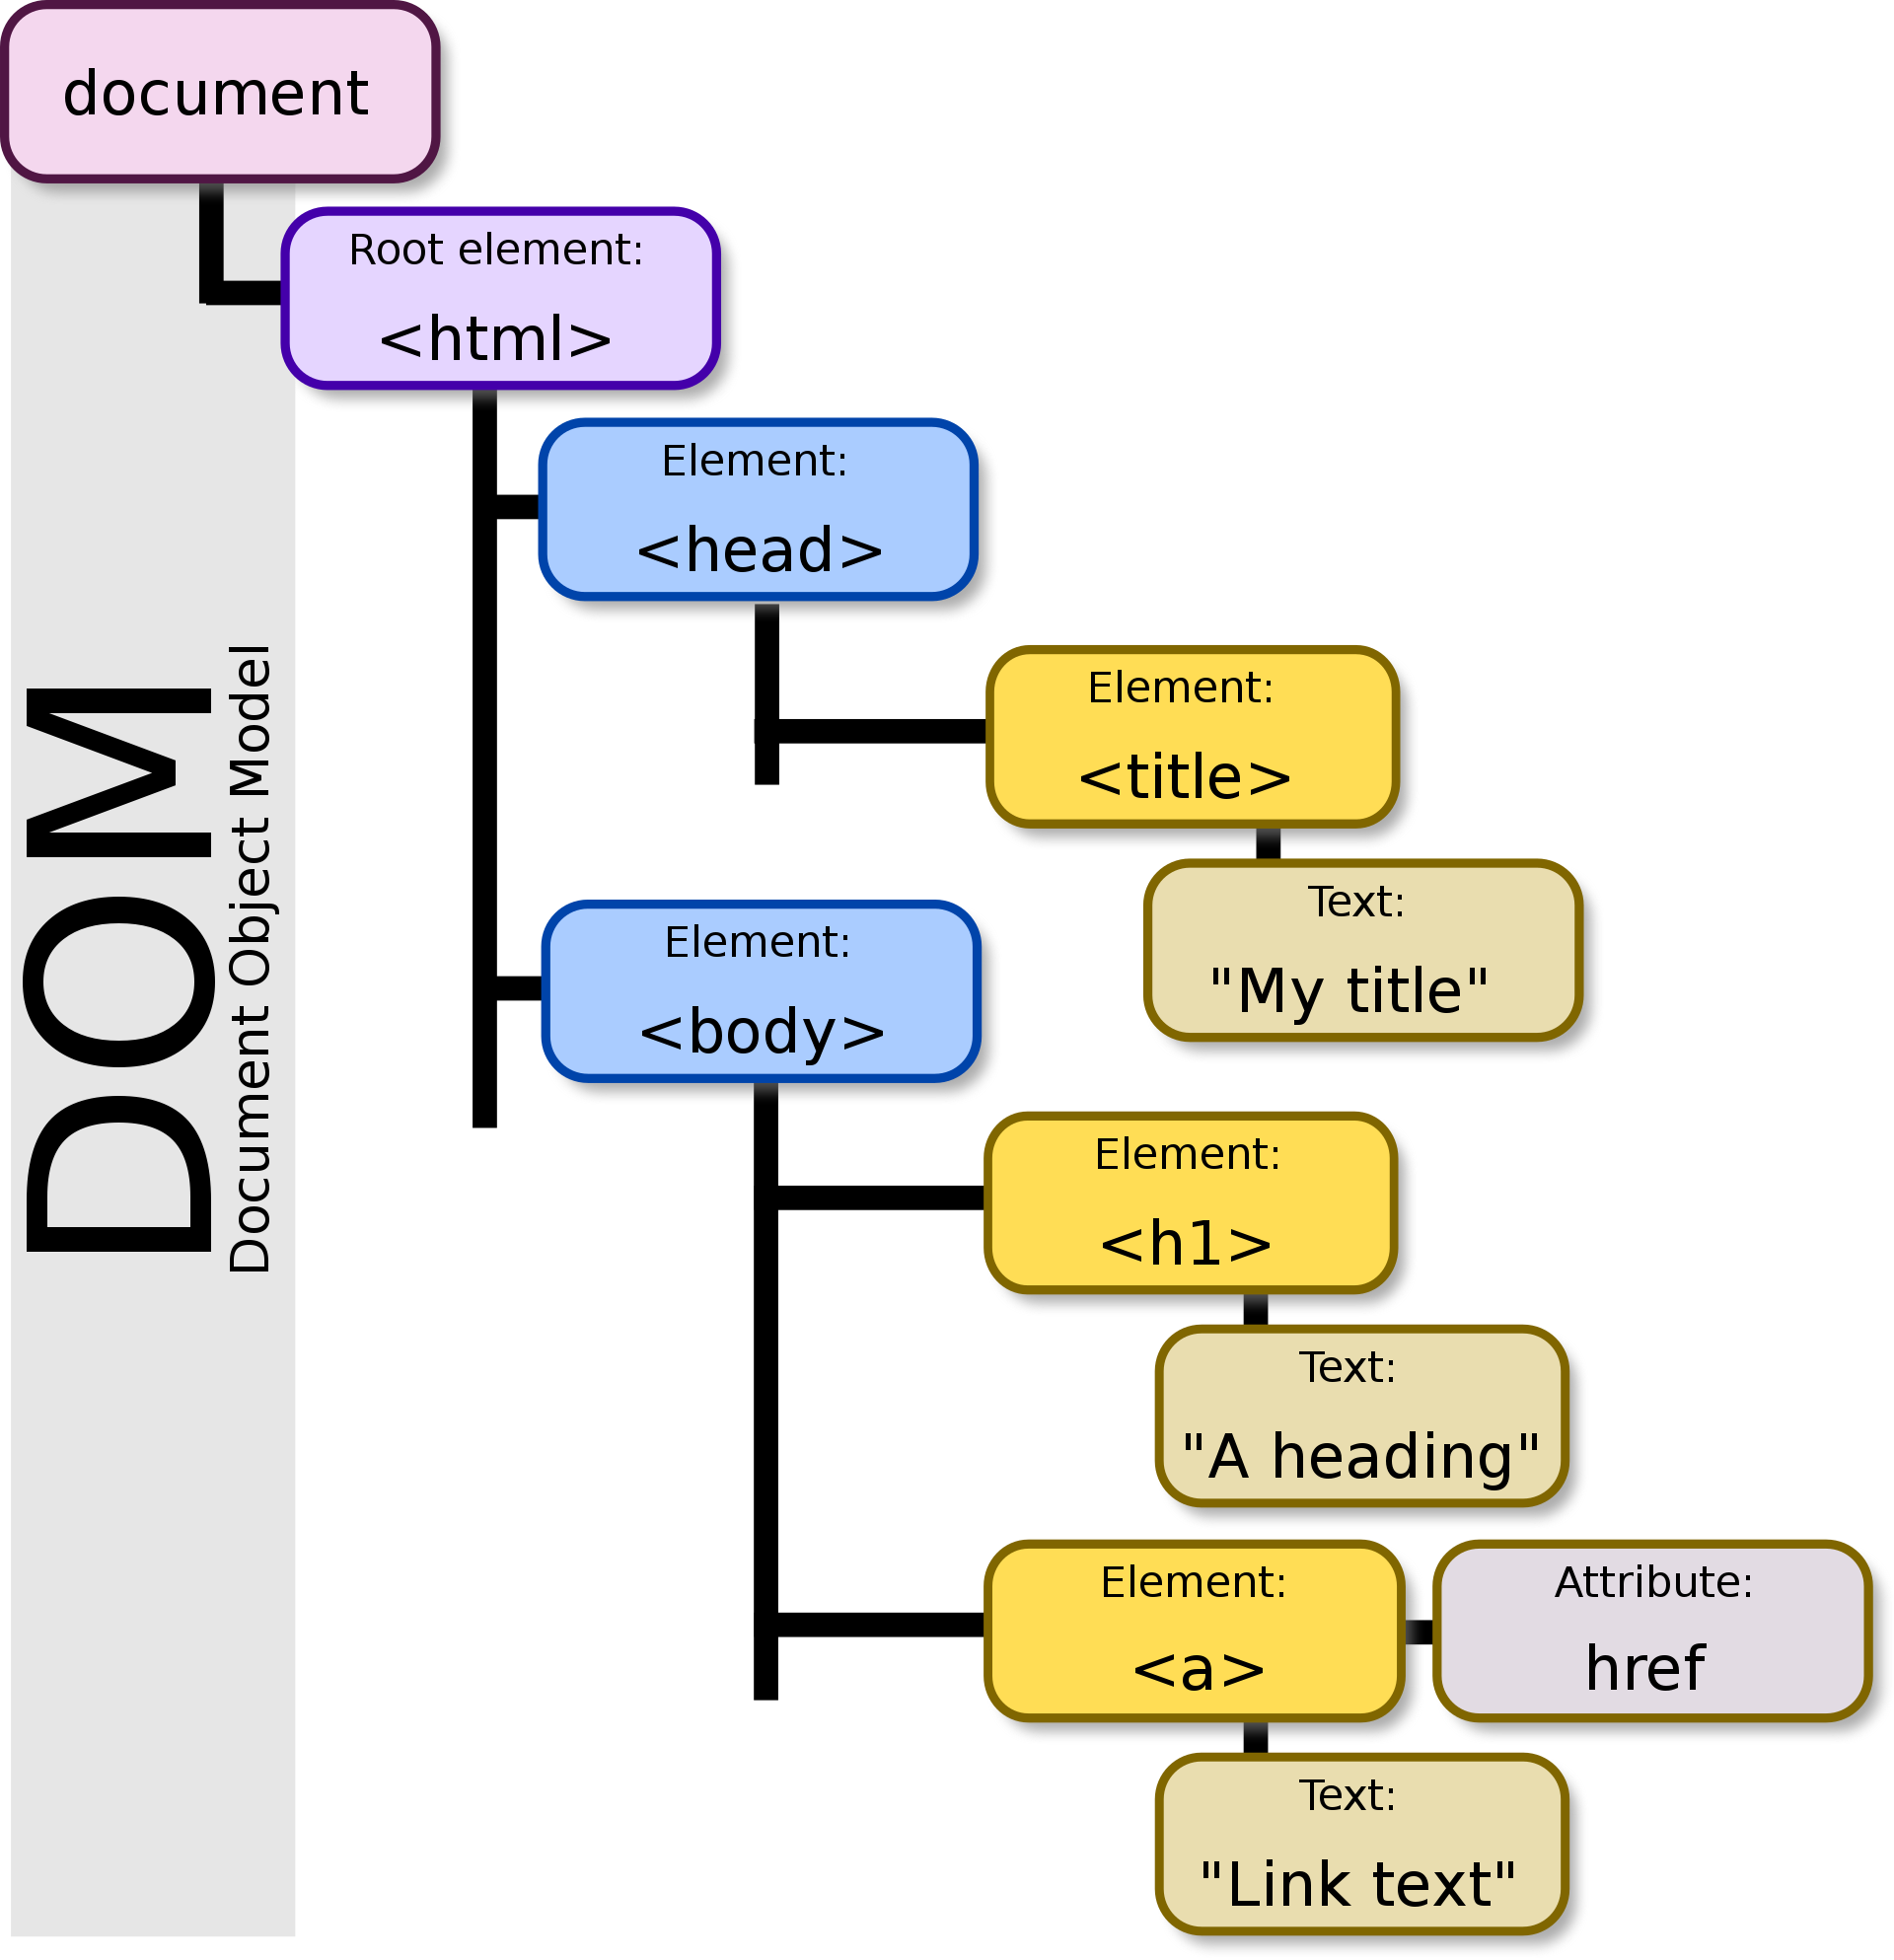
\includegraphics[width=6cm]{ressources/dom.png}
\captionof{figure}{Document Object Model \tiny{\href{https://commons.wikimedia.org/w/index.php?curid=18034500}{source}}}
\label{dom}
\end{center}
\begin{center}
\shadowbox{\parbox{10cm}{\centering Comment implémenter la structure du DOM en Python?}}
\end{center}
\section{Structure arborescente}
\subsection{Élément HTML}
Un élément HTML est constitué d'une paire de \emph{balises} (ouvrante et fermante), d'un \emph{contenu}. De plus la balise peut contenir des attributs.
\begin{center}
\begin{lstlisting}[language=HTML]
<a href="https://cviroulaud.github.io">Un super site</a>
\end{lstlisting}
\captionof{code}{Un lien hypertexte}
\label{lien}
\end{center}
Nous pouvons représenter la balise \emph{a} sous forme d'une structure arborescente (figure \ref{structlien}) et par extension représenter l'ensemble d'une page web.
\begin{center}
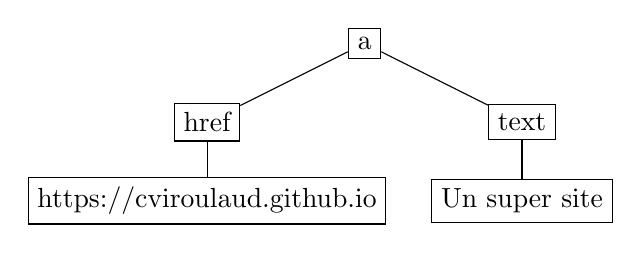
\begin{tikzpicture}
\node[draw] (a) at (0,0) {a};
\node[draw] (href) at (-2,-1) {href};
\node[draw] (text) at (2,-1) {text};
\node[draw] (href2) at (-2,-2) {https://cviroulaud.github.io};
\node[draw] (text2) at (2,-2) {Un super site};
\draw (a) -- (href);
\draw (a) -- (text);
\draw (href) -- (href2);
\draw (text) -- (text2);
\end{tikzpicture}
\captionof{figure}{Structure arborescente d'un lien hypertexte}
\label{structlien}
\end{center}
\subsection{Une page web}
Une page web est une imbrication de balises HTML. La structure arborescente du DOM est évidente.
\begin{center}
\lstinputlisting[language=HTML]{"scripts/premier-site/index.html"}
\captionof{code}{Une page web}
\label{pageweb}
\end{center}
\begin{center}
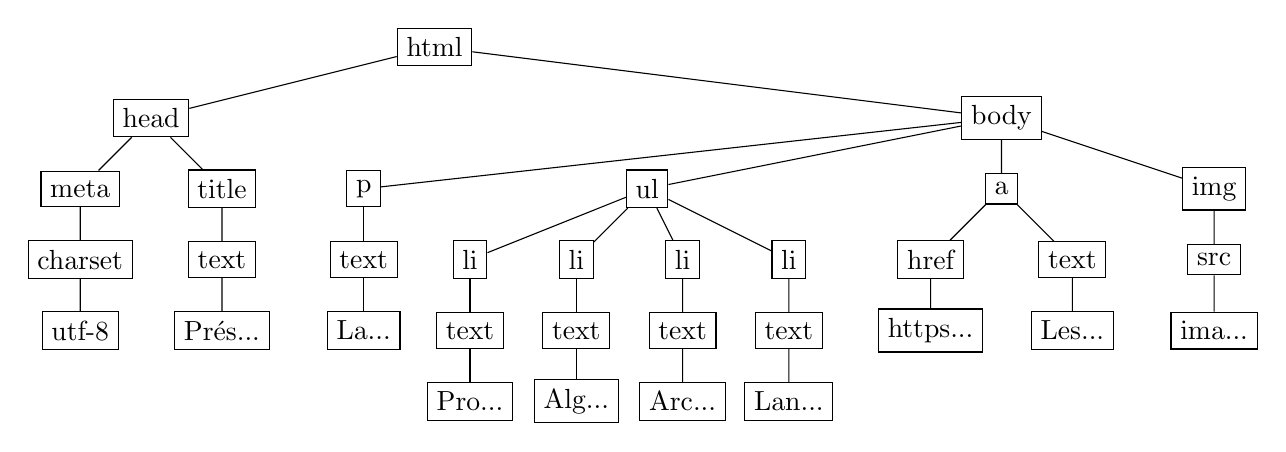
\begin{tikzpicture}[scale=0.9]
\node[draw] (html) at (0,0) {html};
\node[draw] (head) at (-4,-1) {head};
\node[draw] (meta) at (-5,-2) {meta};
\node[draw] (charset) at (-5,-3) {charset};
\node[draw] (charset1) at (-5,-4) {utf-8};
\node[draw] (title) at (-3,-2) {title};
\node[draw] (title1) at (-3,-3) {text};
\node[draw] (title2) at (-3,-4) {Prés...};

\draw (html) -- (head);
\draw (head) -- (meta);
\draw (meta) -- (charset);
\draw (charset) -- (charset1);
\draw (head) -- (title);
\draw (title) -- (title1);
\draw (title2) -- (title1);

\node[draw] (body) at (8,-1) {body};
\node[draw] (p) at (-1,-2) {p};
\node[draw] (p1) at (-1,-3) {text};
\node[draw] (p2) at (-1,-4) {La...};

\node[draw] (ul) at (3,-2) {ul};
\node[draw] (li1) at (0.5,-3) {li};
\node[draw] (li2) at (2,-3) {li};
\node[draw] (li3) at (3.5,-3) {li};
\node[draw] (li4) at (5,-3) {li};
\node[draw] (li1t) at (0.5,-4) {text};
\node[draw] (li2t) at (2,-4) {text};
\node[draw] (li3t) at (3.5,-4) {text};
\node[draw] (li4t) at (5,-4) {text};
\node[draw] (li1t1) at (0.5,-5) {Pro...};
\node[draw] (li2t1) at (2,-5) {Alg...};
\node[draw] (li3t1) at (3.5,-5) {Arc...};
\node[draw] (li4t1) at (5,-5) {Lan...};
\node[draw] (a) at (8,-2) {a};
\node[draw] (href) at (7,-3) {href};
\node[draw] (href1) at (7,-4) {https...};
\node[draw] (atext) at (9,-3) {text};
\node[draw] (atext1) at (9,-4) {Les...};

\node[draw] (img) at (11,-2) {img};
\node[draw] (src) at (11,-3) {src};
\node[draw] (srctext) at (11,-4) {ima...};

\draw (html) -- (body);
\draw (body) -- (p);
\draw (body) -- (ul);
\draw (body) -- (a);
\draw (body) -- (img);
\draw (p) -- (p1);
\draw (p1) -- (p2);
\draw (ul) -- (li1);
\draw (ul) -- (li2);
\draw (ul) -- (li3);
\draw (ul) -- (li4);
\draw (a) -- (href);
\draw (a) -- (atext);
\draw (href) -- (href1);
\draw (atext) -- (atext1);
\draw (img) -- (src);
\draw (src) -- (srctext);
\draw (li1) -- (li1t);
\draw (li1t1) -- (li1t);
\draw (li2) -- (li2t);
\draw (li2t1) -- (li2t);
\draw (li3) -- (li3t);
\draw (li3t1) -- (li3t);
\draw (li4) -- (li4t);
\draw (li4t1) -- (li4t);


\end{tikzpicture}
\captionof{figure}{Structure arborescente d'une page web}
\label{structpage}
\end{center}
\section{Implémentation en Python}
\subsection{Un nœud}
Pour représenter une structure arborescente il est commun d'utiliser la programmation orientée objet.
\begin{center}
\lstinputlisting[firstline=10,lastline=13]{"scripts/dom.py"}
\captionof{code}{Nœud d'une arborescence}
\label{noeud}
\end{center}
Dans le code \ref{noeud} l'attribut \emph{valeur} représente le nom de la balise, l'attribut, le contenu. L'attribut \emph{fils} est la liste des nœuds enfants.\\
Nous pouvons alors construire une représentation du DOM.
\begin{center}
\begin{lstlisting}[language=Python]
dom = Noeud("html", [Noeud("head", []),
                         Noeud("body", []) ])
\end{lstlisting}
\captionof{code}{Représentations des premières balises du DOM}
\label{dom}
\end{center}
\subsection{Manipulation du DOM}
Le \emph{JavaScript} permet d'interagir avec une page web en manipulant le \emph{DOM}. La méthode \emph{Element.getElementsByTagName()} retourne une liste des éléments portant le nom de balise donné. Le DOM étant ici implémenté en Python, il est possible d'imiter le comportement de cette méthode.
\begin{activite}
\begin{enumerate}
\item Télécharger et décompresser \emph{dom-annexe.zip} .
\item Écrire la fonction \emph{récursive} \textbf{taille(dom: Noeud)$\;\rightarrow\;$int} qui renvoie le nombre d'éléments du DOM.
\item Écrire la fonction \emph{récursive}
\begin{center}
\textbf{get\_elements\_by\_tagname(arbre: Noeud, tag: str, res: list)$\;\rightarrow\;$list}
\end{center} qui renvoie la liste \emph{res} des nœuds fils de \emph{tag}.
\end{enumerate}
\end{activite}
\end{Form}
\end{document}